\documentclass[1p]{elsarticle_modified}
%\bibliographystyle{elsarticle-num}

%\usepackage[colorlinks]{hyperref}
%\usepackage{abbrmath_seonhwa} %\Abb, \Ascr, \Acal ,\Abf, \Afrak
\usepackage{amsfonts}
\usepackage{amssymb}
\usepackage{amsmath}
\usepackage{amsthm}
\usepackage{scalefnt}
\usepackage{amsbsy}
\usepackage{kotex}
\usepackage{caption}
\usepackage{subfig}
\usepackage{color}
\usepackage{graphicx}
\usepackage{xcolor} %% white, black, red, green, blue, cyan, magenta, yellow
\usepackage{float}
\usepackage{setspace}
\usepackage{hyperref}

\usepackage{tikz}
\usetikzlibrary{arrows}

\usepackage{multirow}
\usepackage{array} % fixed length table
\usepackage{hhline}

%%%%%%%%%%%%%%%%%%%%%
\makeatletter
\renewcommand*\env@matrix[1][\arraystretch]{%
	\edef\arraystretch{#1}%
	\hskip -\arraycolsep
	\let\@ifnextchar\new@ifnextchar
	\array{*\c@MaxMatrixCols c}}
\makeatother %https://tex.stackexchange.com/questions/14071/how-can-i-increase-the-line-spacing-in-a-matrix
%%%%%%%%%%%%%%%

\usepackage[normalem]{ulem}

\newcommand{\msout}[1]{\ifmmode\text{\sout{\ensuremath{#1}}}\else\sout{#1}\fi}
%SOURCE: \msout is \stkout macro in https://tex.stackexchange.com/questions/20609/strikeout-in-math-mode

\newcommand{\cancel}[1]{
	\ifmmode
	{\color{red}\msout{#1}}
	\else
	{\color{red}\sout{#1}}
	\fi
}

\newcommand{\add}[1]{
	{\color{blue}\uwave{#1}}
}

\newcommand{\replace}[2]{
	\ifmmode
	{\color{red}\msout{#1}}{\color{blue}\uwave{#2}}
	\else
	{\color{red}\sout{#1}}{\color{blue}\uwave{#2}}
	\fi
}

\newcommand{\Sol}{\mathcal{S}} %segment
\newcommand{\D}{D} %diagram
\newcommand{\A}{\mathcal{A}} %arc


%%%%%%%%%%%%%%%%%%%%%%%%%%%%%5 test

\def\sl{\operatorname{\textup{SL}}(2,\Cbb)}
\def\psl{\operatorname{\textup{PSL}}(2,\Cbb)}
\def\quan{\mkern 1mu \triangleright \mkern 1mu}

\theoremstyle{definition}
\newtheorem{thm}{Theorem}[section]
\newtheorem{prop}[thm]{Proposition}
\newtheorem{lem}[thm]{Lemma}
\newtheorem{ques}[thm]{Question}
\newtheorem{cor}[thm]{Corollary}
\newtheorem{defn}[thm]{Definition}
\newtheorem{exam}[thm]{Example}
\newtheorem{rmk}[thm]{Remark}
\newtheorem{alg}[thm]{Algorithm}

\newcommand{\I}{\sqrt{-1}}
\begin{document}

%\begin{frontmatter}
%
%\title{Boundary parabolic representations of knots up to 8 crossings}
%
%%% Group authors per affiliation:
%\author{Yunhi Cho} 
%\address{Department of Mathematics, University of Seoul, Seoul, Korea}
%\ead{yhcho@uos.ac.kr}
%
%
%\author{Seonhwa Kim} %\fnref{s_kim}}
%\address{Center for Geometry and Physics, Institute for Basic Science, Pohang, 37673, Korea}
%\ead{ryeona17@ibs.re.kr}
%
%\author{Hyuk Kim}
%\address{Department of Mathematical Sciences, Seoul National University, Seoul 08826, Korea}
%\ead{hyukkim@snu.ac.kr}
%
%\author{Seokbeom Yoon}
%\address{Department of Mathematical Sciences, Seoul National University, Seoul, 08826,  Korea}
%\ead{sbyoon15@snu.ac.kr}
%
%\begin{abstract}
%We find all boundary parabolic representation of knots up to 8 crossings.
%
%\end{abstract}
%\begin{keyword}
%    \MSC[2010] 57M25 
%\end{keyword}
%
%\end{frontmatter}

%\linenumbers
%\tableofcontents
%
\newcommand\colored[1]{\textcolor{white}{\rule[-0.35ex]{0.8em}{1.4ex}}\kern-0.8em\color{red} #1}%
%\newcommand\colored[1]{\textcolor{white}{ #1}\kern-2.17ex	\textcolor{white}{ #1}\kern-1.81ex	\textcolor{white}{ #1}\kern-2.15ex\color{red}#1	}

{\Large $\underline{11n_{147}~(K11n_{147})}$}

\setlength{\tabcolsep}{10pt}
\renewcommand{\arraystretch}{1.6}
\vspace{1cm}\begin{tabular}{m{100pt}>{\centering\arraybackslash}m{274pt}}
\multirow{5}{120pt}{
	\centering
	\includegraphics[width=112pt]{../../../GIT/diagram.site/Diagrams/png/763_11n_147.png}\\
\ \ \ A knot diagram\footnotemark}&
\allowdisplaybreaks
\textbf{Linearized knot diagam} \\
\cline{2-2}
 &
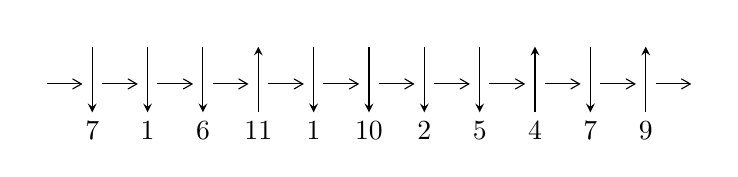
\begin{tikzpicture}[x=20pt, y=17pt]
	% nodes
	\node (C0) at (0, 0) {};
	\node (C1) at (1, 0) {};
	\node (C1U) at (1, +1) {};
	\node (C1D) at (1, -1) {7};

	\node (C2) at (2, 0) {};
	\node (C2U) at (2, +1) {};
	\node (C2D) at (2, -1) {1};

	\node (C3) at (3, 0) {};
	\node (C3U) at (3, +1) {};
	\node (C3D) at (3, -1) {6};

	\node (C4) at (4, 0) {};
	\node (C4U) at (4, +1) {};
	\node (C4D) at (4, -1) {11};

	\node (C5) at (5, 0) {};
	\node (C5U) at (5, +1) {};
	\node (C5D) at (5, -1) {1};

	\node (C6) at (6, 0) {};
	\node (C6U) at (6, +1) {};
	\node (C6D) at (6, -1) {10};

	\node (C7) at (7, 0) {};
	\node (C7U) at (7, +1) {};
	\node (C7D) at (7, -1) {2};

	\node (C8) at (8, 0) {};
	\node (C8U) at (8, +1) {};
	\node (C8D) at (8, -1) {5};

	\node (C9) at (9, 0) {};
	\node (C9U) at (9, +1) {};
	\node (C9D) at (9, -1) {4};

	\node (C10) at (10, 0) {};
	\node (C10U) at (10, +1) {};
	\node (C10D) at (10, -1) {7};

	\node (C11) at (11, 0) {};
	\node (C11U) at (11, +1) {};
	\node (C11D) at (11, -1) {9};
	\node (C12) at (12, 0) {};

	% arrows
	\draw[->,>={angle 60}]
	(C0) edge (C1) (C1) edge (C2) (C2) edge (C3) (C3) edge (C4) (C4) edge (C5) (C5) edge (C6) (C6) edge (C7) (C7) edge (C8) (C8) edge (C9) (C9) edge (C10) (C10) edge (C11) (C11) edge (C12) ;	\draw[->,>=stealth]
	(C1U) edge (C1D) (C2U) edge (C2D) (C3U) edge (C3D) (C4D) edge (C4U) (C5U) edge (C5D) (C6U) edge (C6D) (C7U) edge (C7D) (C8U) edge (C8D) (C9D) edge (C9U) (C10U) edge (C10D) (C11D) edge (C11U) ;
	\end{tikzpicture} \\
\hhline{~~} \\& 
\textbf{Solving Sequence} \\ \cline{2-2} 
 &
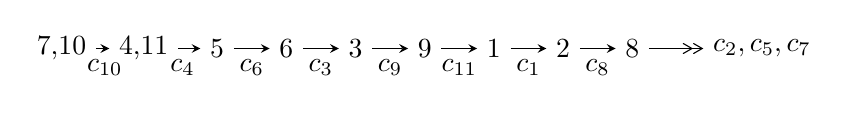
\begin{tikzpicture}[x=25pt, y=7pt]
	% node
	\node (A0) at (-1/8, 0) {7,10};
	\node (A1) at (17/16, 0) {4,11};
	\node (A2) at (17/8, 0) {5};
	\node (A3) at (25/8, 0) {6};
	\node (A4) at (33/8, 0) {3};
	\node (A5) at (41/8, 0) {9};
	\node (A6) at (49/8, 0) {1};
	\node (A7) at (57/8, 0) {2};
	\node (A8) at (65/8, 0) {8};
	\node (C1) at (1/2, -1) {$c_{10}$};
	\node (C2) at (13/8, -1) {$c_{4}$};
	\node (C3) at (21/8, -1) {$c_{6}$};
	\node (C4) at (29/8, -1) {$c_{3}$};
	\node (C5) at (37/8, -1) {$c_{9}$};
	\node (C6) at (45/8, -1) {$c_{11}$};
	\node (C7) at (53/8, -1) {$c_{1}$};
	\node (C8) at (61/8, -1) {$c_{8}$};
	\node (A9) at (10, 0) {$c_{2},c_{5},c_{7}$};

	% edge
	\draw[->,>=stealth]	
	(A0) edge (A1) (A1) edge (A2) (A2) edge (A3) (A3) edge (A4) (A4) edge (A5) (A5) edge (A6) (A6) edge (A7) (A7) edge (A8) ;
	\draw[->>,>={angle 60}]	
	(A8) edge (A9);
\end{tikzpicture} \\ 

\end{tabular} \\

\footnotetext{
The image of knot diagram is generated by the software ``\textbf{Draw programme}" developed by Andrew Bartholomew(\url{http://www.layer8.co.uk/maths/draw/index.htm\#Running-draw}), where we modified some parts for our purpose(\url{https://github.com/CATsTAILs/LinksPainter}).
}\phantom \\ \newline 
\centering \textbf{Ideals for irreducible components\footnotemark of $X_{\text{par}}$} 
 
\begin{align*}
I^u_{1}&=\langle 
1.98756\times10^{46} u^{32}+1.28266\times10^{46} u^{31}+\cdots+1.35435\times10^{47} b+2.77751\times10^{46},\\
\phantom{I^u_{1}}&\phantom{= \langle  }2.97484\times10^{47} u^{32}+3.19635\times10^{47} u^{31}+\cdots+1.35435\times10^{47} a+4.86114\times10^{48},\;u^{33}+u^{32}+\cdots+14 u+1\rangle \\
I^u_{2}&=\langle 
u^{14}-3 u^{12}- u^{11}+u^{10}+2 u^9+7 u^8-4 u^7-11 u^6+4 u^5+6 u^4-5 u^3- u^2+b,\\
\phantom{I^u_{2}}&\phantom{= \langle  }-73 u^{14}+113 u^{13}+\cdots+19 a+238,\\
\phantom{I^u_{2}}&\phantom{= \langle  }u^{15}-4 u^{13}- u^{12}+4 u^{11}+3 u^{10}+6 u^9-6 u^8-18 u^7+8 u^6+17 u^5-9 u^4-7 u^3+5 u^2+u-1\rangle \\
\\
\end{align*}
\raggedright * 2 irreducible components of $\dim_{\mathbb{C}}=0$, with total 48 representations.\\
\footnotetext{All coefficients of polynomials are rational numbers. But the coefficients are sometimes approximated in decimal forms when there is not enough margin.}
\newpage
\renewcommand{\arraystretch}{1}
\centering \section*{I. $I^u_{1}= \langle 1.99\times10^{46} u^{32}+1.28\times10^{46} u^{31}+\cdots+1.35\times10^{47} b+2.78\times10^{46},\;2.97\times10^{47} u^{32}+3.20\times10^{47} u^{31}+\cdots+1.35\times10^{47} a+4.86\times10^{48},\;u^{33}+u^{32}+\cdots+14 u+1 \rangle$}
\flushleft \textbf{(i) Arc colorings}\\
\begin{tabular}{m{7pt} m{180pt} m{7pt} m{180pt} }
\flushright $a_{7}=$&$\begin{pmatrix}0\\u\end{pmatrix}$ \\
\flushright $a_{10}=$&$\begin{pmatrix}1\\0\end{pmatrix}$ \\
\flushright $a_{4}=$&$\begin{pmatrix}-2.19651 u^{32}-2.36006 u^{31}+\cdots-288.611 u-35.8928\\-0.146754 u^{32}-0.0947065 u^{31}+\cdots-10.0032 u-0.205081\end{pmatrix}$ \\
\flushright $a_{11}=$&$\begin{pmatrix}1\\u^2\end{pmatrix}$ \\
\flushright $a_{5}=$&$\begin{pmatrix}-2.39829 u^{32}-2.50756 u^{31}+\cdots-303.100 u-36.2614\\-0.153523 u^{32}-0.103389 u^{31}+\cdots-10.5613 u-0.259363\end{pmatrix}$ \\
\flushright $a_{6}=$&$\begin{pmatrix}u\\u\end{pmatrix}$ \\
\flushright $a_{3}=$&$\begin{pmatrix}-2.25912 u^{32}-2.42484 u^{31}+\cdots-293.679 u-36.1084\\-0.209360 u^{32}-0.159488 u^{31}+\cdots-15.0713 u-0.420679\end{pmatrix}$ \\
\flushright $a_{9}=$&$\begin{pmatrix}1.41506 u^{32}+1.04966 u^{31}+\cdots+69.0722 u-12.5718\\-0.0802570 u^{32}-0.116578 u^{31}+\cdots-12.6183 u-1.15166\end{pmatrix}$ \\
\flushright $a_{1}=$&$\begin{pmatrix}-1.63104 u^{32}-1.63496 u^{31}+\cdots-199.736 u-22.5435\\-0.0316774 u^{32}-0.0129877 u^{31}+\cdots-6.21518 u-0.0761096\end{pmatrix}$ \\
\flushright $a_{2}=$&$\begin{pmatrix}-1.63104 u^{32}-1.63496 u^{31}+\cdots-199.736 u-22.5435\\-0.00657502 u^{32}-0.00502953 u^{31}+\cdots-4.52928 u-0.0721915\end{pmatrix}$ \\
\flushright $a_{8}=$&$\begin{pmatrix}2.50333 u^{32}+2.57261 u^{31}+\cdots+314.930 u+36.4507\\0.0683064 u^{32}+0.0388114 u^{31}+\cdots+8.35580 u+0.120011\end{pmatrix}$\\ \flushright $a_{8}=$&$\begin{pmatrix}2.50333 u^{32}+2.57261 u^{31}+\cdots+314.930 u+36.4507\\0.0683064 u^{32}+0.0388114 u^{31}+\cdots+8.35580 u+0.120011\end{pmatrix}$\\&\end{tabular}
\flushleft \textbf{(ii) Obstruction class $= -1$}\\~\\
\flushleft \textbf{(iii) Cusp Shapes $= 1.80265 u^{32}+1.77164 u^{31}+\cdots+131.190 u-2.63139$}\\~\\
\newpage\renewcommand{\arraystretch}{1}
\flushleft \textbf{(iv) u-Polynomials at the component}\newline \\
\begin{tabular}{m{50pt}|m{274pt}}
Crossings & \hspace{64pt}u-Polynomials at each crossing \\
\hline $$\begin{aligned}c_{1},c_{7}\end{aligned}$$&$\begin{aligned}
&u^{33}- u^{32}+\cdots-377 u+49
\end{aligned}$\\
\hline $$\begin{aligned}c_{2}\end{aligned}$$&$\begin{aligned}
&u^{33}+51 u^{32}+\cdots-6243 u+2401
\end{aligned}$\\
\hline $$\begin{aligned}c_{3}\end{aligned}$$&$\begin{aligned}
&u^{33}+4 u^{32}+\cdots+1014 u+53
\end{aligned}$\\
\hline $$\begin{aligned}c_{4}\end{aligned}$$&$\begin{aligned}
&u^{33}-3 u^{32}+\cdots+143 u+167
\end{aligned}$\\
\hline $$\begin{aligned}c_{5}\end{aligned}$$&$\begin{aligned}
&u^{33}-31 u^{31}+\cdots+31219 u+7513
\end{aligned}$\\
\hline $$\begin{aligned}c_{6},c_{10}\end{aligned}$$&$\begin{aligned}
&u^{33}+u^{32}+\cdots+14 u+1
\end{aligned}$\\
\hline $$\begin{aligned}c_{8}\end{aligned}$$&$\begin{aligned}
&u^{33}+3 u^{32}+\cdots+43957 u+23657
\end{aligned}$\\
\hline $$\begin{aligned}c_{9}\end{aligned}$$&$\begin{aligned}
&u^{33}+u^{32}+\cdots-194 u+69
\end{aligned}$\\
\hline $$\begin{aligned}c_{11}\end{aligned}$$&$\begin{aligned}
&u^{33}+2 u^{32}+\cdots+12 u+1
\end{aligned}$\\
\hline
\end{tabular}\\~\\
\newpage\renewcommand{\arraystretch}{1}
\flushleft \textbf{(v) Riley Polynomials at the component}\newline \\
\begin{tabular}{m{50pt}|m{274pt}}
Crossings & \hspace{64pt}Riley Polynomials at each crossing \\
\hline $$\begin{aligned}c_{1},c_{7}\end{aligned}$$&$\begin{aligned}
&y^{33}-51 y^{32}+\cdots-6243 y-2401
\end{aligned}$\\
\hline $$\begin{aligned}c_{2}\end{aligned}$$&$\begin{aligned}
&y^{33}-127 y^{32}+\cdots-823598607 y-5764801
\end{aligned}$\\
\hline $$\begin{aligned}c_{3}\end{aligned}$$&$\begin{aligned}
&y^{33}-62 y^{32}+\cdots+1267120 y-2809
\end{aligned}$\\
\hline $$\begin{aligned}c_{4}\end{aligned}$$&$\begin{aligned}
&y^{33}+13 y^{32}+\cdots+203815 y-27889
\end{aligned}$\\
\hline $$\begin{aligned}c_{5}\end{aligned}$$&$\begin{aligned}
&y^{33}-62 y^{32}+\cdots-187379697 y-56445169
\end{aligned}$\\
\hline $$\begin{aligned}c_{6},c_{10}\end{aligned}$$&$\begin{aligned}
&y^{33}-31 y^{32}+\cdots-58 y-1
\end{aligned}$\\
\hline $$\begin{aligned}c_{8}\end{aligned}$$&$\begin{aligned}
&y^{33}-35 y^{32}+\cdots+2107894731 y-559653649
\end{aligned}$\\
\hline $$\begin{aligned}c_{9}\end{aligned}$$&$\begin{aligned}
&y^{33}+13 y^{32}+\cdots-3488 y-4761
\end{aligned}$\\
\hline $$\begin{aligned}c_{11}\end{aligned}$$&$\begin{aligned}
&y^{33}+4 y^{32}+\cdots+94 y-1
\end{aligned}$\\
\hline
\end{tabular}\\~\\
\newpage\flushleft \textbf{(vi) Complex Volumes and Cusp Shapes}
$$\begin{array}{c|c|c}  
\text{Solutions to }I^u_{1}& \I (\text{vol} + \sqrt{-1}CS) & \text{Cusp shape}\\
 \hline 
\begin{aligned}
u &= \phantom{-}1.127190 + 0.291980 I \\
a &= \phantom{-}0.90634 + 1.24177 I \\
b &= -0.280294 + 0.848945 I\end{aligned}
 & -4.91531 - 2.57543 I & -14.7490 + 3.5042 I \\ \hline\begin{aligned}
u &= \phantom{-}1.127190 - 0.291980 I \\
a &= \phantom{-}0.90634 - 1.24177 I \\
b &= -0.280294 - 0.848945 I\end{aligned}
 & -4.91531 + 2.57543 I & -14.7490 - 3.5042 I \\ \hline\begin{aligned}
u &= -0.258449 + 1.156160 I \\
a &= \phantom{-}0.118269 + 0.247166 I \\
b &= \phantom{-}0.381205 - 0.236102 I\end{aligned}
 & \phantom{-}2.26695 + 2.07000 I & \phantom{-}4.04253 + 2.66758 I \\ \hline\begin{aligned}
u &= -0.258449 - 1.156160 I \\
a &= \phantom{-}0.118269 - 0.247166 I \\
b &= \phantom{-}0.381205 + 0.236102 I\end{aligned}
 & \phantom{-}2.26695 - 2.07000 I & \phantom{-}4.04253 - 2.66758 I \\ \hline\begin{aligned}
u &= -1.214840 + 0.304735 I \\
a &= -0.676508 + 1.000140 I \\
b &= -0.363295 + 1.180830 I\end{aligned}
 & -2.65106 + 0.57067 I & -7.43301 + 1.59468 I \\ \hline\begin{aligned}
u &= -1.214840 - 0.304735 I \\
a &= -0.676508 - 1.000140 I \\
b &= -0.363295 - 1.180830 I\end{aligned}
 & -2.65106 - 0.57067 I & -7.43301 - 1.59468 I \\ \hline\begin{aligned}
u &= -1.203030 + 0.458288 I \\
a &= -0.26246 + 1.71772 I \\
b &= \phantom{-}1.23330 + 1.31569 I\end{aligned}
 & -4.39762 + 3.59048 I & -13.6557 - 4.4501 I \\ \hline\begin{aligned}
u &= -1.203030 - 0.458288 I \\
a &= -0.26246 - 1.71772 I \\
b &= \phantom{-}1.23330 - 1.31569 I\end{aligned}
 & -4.39762 - 3.59048 I & -13.6557 + 4.4501 I \\ \hline\begin{aligned}
u &= \phantom{-}1.235800 + 0.362699 I \\
a &= -0.03086 + 1.63923 I \\
b &= -0.508343 + 0.929615 I\end{aligned}
 & -1.99613 - 4.92165 I & -6.31797 + 5.98553 I \\ \hline\begin{aligned}
u &= \phantom{-}1.235800 - 0.362699 I \\
a &= -0.03086 - 1.63923 I \\
b &= -0.508343 - 0.929615 I\end{aligned}
 & -1.99613 + 4.92165 I & -6.31797 - 5.98553 I\\
 \hline 
 \end{array}$$\newpage$$\begin{array}{c|c|c}  
\text{Solutions to }I^u_{1}& \I (\text{vol} + \sqrt{-1}CS) & \text{Cusp shape}\\
 \hline 
\begin{aligned}
u &= -0.569481\phantom{ +0.000000I} \\
a &= -0.688600\phantom{ +0.000000I} \\
b &= -0.604199\phantom{ +0.000000I}\end{aligned}
 & -1.00066\phantom{ +0.000000I} & -10.2820\phantom{ +0.000000I} \\ \hline\begin{aligned}
u &= -0.173547 + 0.479626 I \\
a &= -0.525769 - 0.734371 I \\
b &= -0.526827 + 0.796028 I\end{aligned}
 & -1.45039 + 0.21379 I & -8.69019 - 1.03252 I \\ \hline\begin{aligned}
u &= -0.173547 - 0.479626 I \\
a &= -0.525769 + 0.734371 I \\
b &= -0.526827 - 0.796028 I\end{aligned}
 & -1.45039 - 0.21379 I & -8.69019 + 1.03252 I \\ \hline\begin{aligned}
u &= \phantom{-}0.129625 + 0.488487 I \\
a &= -0.477469 + 0.473795 I \\
b &= \phantom{-}0.889420 + 0.379105 I\end{aligned}
 & \phantom{-}1.34993 + 1.55576 I & \phantom{-}0.80167 - 1.35691 I \\ \hline\begin{aligned}
u &= \phantom{-}0.129625 - 0.488487 I \\
a &= -0.477469 - 0.473795 I \\
b &= \phantom{-}0.889420 - 0.379105 I\end{aligned}
 & \phantom{-}1.34993 - 1.55576 I & \phantom{-}0.80167 + 1.35691 I \\ \hline\begin{aligned}
u &= -1.52232 + 0.04381 I \\
a &= -0.703268 - 0.941307 I \\
b &= \phantom{-}0.711491 - 0.715800 I\end{aligned}
 & -14.5102 - 1.0864 I & -12.76434 + 6.06201 I \\ \hline\begin{aligned}
u &= -1.52232 - 0.04381 I \\
a &= -0.703268 + 0.941307 I \\
b &= \phantom{-}0.711491 + 0.715800 I\end{aligned}
 & -14.5102 + 1.0864 I & -12.76434 - 6.06201 I \\ \hline\begin{aligned}
u &= -0.078681 + 0.424703 I \\
a &= -0.651126 + 0.856956 I \\
b &= -0.868396 - 0.574824 I\end{aligned}
 & \phantom{-}0.04954 + 4.46270 I & -2.71293 - 8.43854 I \\ \hline\begin{aligned}
u &= -0.078681 - 0.424703 I \\
a &= -0.651126 - 0.856956 I \\
b &= -0.868396 + 0.574824 I\end{aligned}
 & \phantom{-}0.04954 - 4.46270 I & -2.71293 + 8.43854 I \\ \hline\begin{aligned}
u &= \phantom{-}1.59376 + 0.04874 I \\
a &= -0.476576 - 0.859038 I \\
b &= -1.93979 - 1.30100 I\end{aligned}
 & -15.3428 - 2.1802 I & \phantom{-0.000000 } 0\\
 \hline 
 \end{array}$$\newpage$$\begin{array}{c|c|c}  
\text{Solutions to }I^u_{1}& \I (\text{vol} + \sqrt{-1}CS) & \text{Cusp shape}\\
 \hline 
\begin{aligned}
u &= \phantom{-}1.59376 - 0.04874 I \\
a &= -0.476576 + 0.859038 I \\
b &= -1.93979 + 1.30100 I\end{aligned}
 & -15.3428 + 2.1802 I & \phantom{-0.000000 } 0 \\ \hline\begin{aligned}
u &= \phantom{-}1.62635 + 0.11374 I \\
a &= \phantom{-}0.254364 - 1.108810 I \\
b &= \phantom{-}0.80851 - 1.54572 I\end{aligned}
 & -6.41445 - 6.00796 I & \phantom{-0.000000 } 0 \\ \hline\begin{aligned}
u &= \phantom{-}1.62635 - 0.11374 I \\
a &= \phantom{-}0.254364 + 1.108810 I \\
b &= \phantom{-}0.80851 + 1.54572 I\end{aligned}
 & -6.41445 + 6.00796 I & \phantom{-0.000000 } 0 \\ \hline\begin{aligned}
u &= -1.65170 + 0.20395 I \\
a &= \phantom{-}0.329105 - 0.879132 I \\
b &= -0.047223 - 1.078280 I\end{aligned}
 & -5.75926 - 1.26707 I & \phantom{-0.000000 } 0 \\ \hline\begin{aligned}
u &= -1.65170 - 0.20395 I \\
a &= \phantom{-}0.329105 + 0.879132 I \\
b &= -0.047223 + 1.078280 I\end{aligned}
 & -5.75926 + 1.26707 I & \phantom{-0.000000 } 0 \\ \hline\begin{aligned}
u &= \phantom{-}0.17496 + 1.66747 I \\
a &= -0.0254572 - 0.0404340 I \\
b &= \phantom{-}0.312479 - 1.241810 I\end{aligned}
 & -11.57590 - 4.55852 I & \phantom{-0.000000 } 0 \\ \hline\begin{aligned}
u &= \phantom{-}0.17496 - 1.66747 I \\
a &= -0.0254572 + 0.0404340 I \\
b &= \phantom{-}0.312479 + 1.241810 I\end{aligned}
 & -11.57590 + 4.55852 I & \phantom{-0.000000 } 0 \\ \hline\begin{aligned}
u &= -1.65356 + 0.67060 I \\
a &= \phantom{-}0.202508 - 1.183540 I \\
b &= -1.06866 - 1.49216 I\end{aligned}
 & -17.3332 + 12.6517 I & \phantom{-0.000000 } 0 \\ \hline\begin{aligned}
u &= -1.65356 - 0.67060 I \\
a &= \phantom{-}0.202508 + 1.183540 I \\
b &= -1.06866 + 1.49216 I\end{aligned}
 & -17.3332 - 12.6517 I & \phantom{-0.000000 } 0 \\ \hline\begin{aligned}
u &= -0.0667735 + 0.0884449 I \\
a &= -16.3648 - 15.7170 I \\
b &= \phantom{-}0.429817 - 0.686138 I\end{aligned}
 & -9.04777 + 1.61427 I & -11.19487 + 6.80933 I\\
 \hline 
 \end{array}$$\newpage$$\begin{array}{c|c|c}  
\text{Solutions to }I^u_{1}& \I (\text{vol} + \sqrt{-1}CS) & \text{Cusp shape}\\
 \hline 
\begin{aligned}
u &= -0.0667735 - 0.0884449 I \\
a &= -16.3648 + 15.7170 I \\
b &= \phantom{-}0.429817 + 0.686138 I\end{aligned}
 & -9.04777 - 1.61427 I & -11.19487 - 6.80933 I \\ \hline\begin{aligned}
u &= \phantom{-}1.71996 + 0.81176 I \\
a &= -0.271982 - 0.744516 I \\
b &= \phantom{-}0.638698 - 1.235990 I\end{aligned}
 & -16.3377 - 4.4651 I & \phantom{-0.000000 } 0 \\ \hline\begin{aligned}
u &= \phantom{-}1.71996 - 0.81176 I \\
a &= -0.271982 + 0.744516 I \\
b &= \phantom{-}0.638698 + 1.235990 I\end{aligned}
 & -16.3377 + 4.4651 I & \phantom{-0.000000 } 0\\
 \hline 
 \end{array}$$\newpage\newpage\renewcommand{\arraystretch}{1}
\centering \section*{II. $I^u_{2}= \langle u^{14}-3 u^{12}+\cdots- u^2+b,\;-73 u^{14}+113 u^{13}+\cdots+19 a+238,\;u^{15}-4 u^{13}+\cdots+u-1 \rangle$}
\flushleft \textbf{(i) Arc colorings}\\
\begin{tabular}{m{7pt} m{180pt} m{7pt} m{180pt} }
\flushright $a_{7}=$&$\begin{pmatrix}0\\u\end{pmatrix}$ \\
\flushright $a_{10}=$&$\begin{pmatrix}1\\0\end{pmatrix}$ \\
\flushright $a_{4}=$&$\begin{pmatrix}3.84211 u^{14}-5.94737 u^{13}+\cdots+24.1053 u-12.5263\\- u^{14}+3 u^{12}+\cdots+5 u^3+u^2\end{pmatrix}$ \\
\flushright $a_{11}=$&$\begin{pmatrix}1\\u^2\end{pmatrix}$ \\
\flushright $a_{5}=$&$\begin{pmatrix}0.526316 u^{14}-3.84211 u^{13}+\cdots+14.3158 u-6.57895\\-3.36842 u^{14}+0.789474 u^{13}+\cdots-5.42105 u+2.10526\end{pmatrix}$ \\
\flushright $a_{6}=$&$\begin{pmatrix}u\\u\end{pmatrix}$ \\
\flushright $a_{3}=$&$\begin{pmatrix}0.526316 u^{14}-3.84211 u^{13}+\cdots+13.3158 u-6.57895\\-4.31579 u^{14}+2.10526 u^{13}+\cdots-10.7895 u+5.94737\end{pmatrix}$ \\
\flushright $a_{9}=$&$\begin{pmatrix}-9.31579 u^{14}+4.10526 u^{13}+\cdots-29.7895 u+8.94737\\-3 u^{13}+10 u^{11}+\cdots+4 u-4\end{pmatrix}$ \\
\flushright $a_{1}=$&$\begin{pmatrix}-0.526316 u^{14}+3.84211 u^{13}+\cdots-9.31579 u+7.57895\\-5.47368 u^{14}+8.15789 u^{13}+\cdots-28.6842 u+17.4211\end{pmatrix}$ \\
\flushright $a_{2}=$&$\begin{pmatrix}-0.526316 u^{14}+3.84211 u^{13}+\cdots-9.31579 u+7.57895\\-6.42105 u^{14}+9.47368 u^{13}+\cdots-33.0526 u+21.2632\end{pmatrix}$ \\
\flushright $a_{8}=$&$\begin{pmatrix}3.94737 u^{14}-4.31579 u^{13}+\cdots+14.3684 u-10.8421\\6.57895 u^{14}-10.5263 u^{13}+\cdots+36.9474 u-21.7368\end{pmatrix}$\\ \flushright $a_{8}=$&$\begin{pmatrix}3.94737 u^{14}-4.31579 u^{13}+\cdots+14.3684 u-10.8421\\6.57895 u^{14}-10.5263 u^{13}+\cdots+36.9474 u-21.7368\end{pmatrix}$\\&\end{tabular}
\flushleft \textbf{(ii) Obstruction class $= 1$}\\~\\
\flushleft \textbf{(iii) Cusp Shapes $= -\frac{124}{19} u^{14}+\frac{301}{19} u^{13}+\frac{478}{19} u^{12}-\frac{941}{19} u^{11}-\frac{746}{19} u^{10}+\frac{339}{19} u^9-\frac{2}{19} u^8+\frac{2898}{19} u^7+\frac{696}{19} u^6-\frac{5366}{19} u^5-\frac{218}{19} u^4+\frac{4007}{19} u^3-\frac{1063}{19} u^2-\frac{1032}{19} u+\frac{296}{19}$}\\~\\
\newpage\renewcommand{\arraystretch}{1}
\flushleft \textbf{(iv) u-Polynomials at the component}\newline \\
\begin{tabular}{m{50pt}|m{274pt}}
Crossings & \hspace{64pt}u-Polynomials at each crossing \\
\hline $$\begin{aligned}c_{1}\end{aligned}$$&$\begin{aligned}
&u^{15}-8 u^{13}+\cdots-4 u-1
\end{aligned}$\\
\hline $$\begin{aligned}c_{2}\end{aligned}$$&$\begin{aligned}
&u^{15}+16 u^{14}+\cdots+18 u+1
\end{aligned}$\\
\hline $$\begin{aligned}c_{3}\end{aligned}$$&$\begin{aligned}
&u^{15}-11 u^{14}+\cdots+73 u-19
\end{aligned}$\\
\hline $$\begin{aligned}c_{4}\end{aligned}$$&$\begin{aligned}
&u^{15}-2 u^{13}+\cdots-2 u-1
\end{aligned}$\\
\hline $$\begin{aligned}c_{5}\end{aligned}$$&$\begin{aligned}
&u^{15}- u^{14}+\cdots-4 u-1
\end{aligned}$\\
\hline $$\begin{aligned}c_{6}\end{aligned}$$&$\begin{aligned}
&u^{15}-4 u^{13}+\cdots+u+1
\end{aligned}$\\
\hline $$\begin{aligned}c_{7}\end{aligned}$$&$\begin{aligned}
&u^{15}-8 u^{13}+\cdots-4 u+1
\end{aligned}$\\
\hline $$\begin{aligned}c_{8}\end{aligned}$$&$\begin{aligned}
&u^{15}-2 u^{13}+\cdots+2 u+1
\end{aligned}$\\
\hline $$\begin{aligned}c_{9}\end{aligned}$$&$\begin{aligned}
&u^{15}+2 u^{12}+3 u^{10}+4 u^8+6 u^7-6 u^6+10 u^5+5 u^4-2 u^3+6 u^2- u+1
\end{aligned}$\\
\hline $$\begin{aligned}c_{10}\end{aligned}$$&$\begin{aligned}
&u^{15}-4 u^{13}+\cdots+u-1
\end{aligned}$\\
\hline $$\begin{aligned}c_{11}\end{aligned}$$&$\begin{aligned}
&u^{15}-3 u^{14}+\cdots+3 u+1
\end{aligned}$\\
\hline
\end{tabular}\\~\\
\newpage\renewcommand{\arraystretch}{1}
\flushleft \textbf{(v) Riley Polynomials at the component}\newline \\
\begin{tabular}{m{50pt}|m{274pt}}
Crossings & \hspace{64pt}Riley Polynomials at each crossing \\
\hline $$\begin{aligned}c_{1},c_{7}\end{aligned}$$&$\begin{aligned}
&y^{15}-16 y^{14}+\cdots+18 y-1
\end{aligned}$\\
\hline $$\begin{aligned}c_{2}\end{aligned}$$&$\begin{aligned}
&y^{15}-24 y^{14}+\cdots+2 y-1
\end{aligned}$\\
\hline $$\begin{aligned}c_{3}\end{aligned}$$&$\begin{aligned}
&y^{15}-19 y^{14}+\cdots+1529 y-361
\end{aligned}$\\
\hline $$\begin{aligned}c_{4}\end{aligned}$$&$\begin{aligned}
&y^{15}-4 y^{14}+\cdots-12 y-1
\end{aligned}$\\
\hline $$\begin{aligned}c_{5}\end{aligned}$$&$\begin{aligned}
&y^{15}-7 y^{14}+\cdots-8 y-1
\end{aligned}$\\
\hline $$\begin{aligned}c_{6},c_{10}\end{aligned}$$&$\begin{aligned}
&y^{15}-8 y^{14}+\cdots+11 y-1
\end{aligned}$\\
\hline $$\begin{aligned}c_{8}\end{aligned}$$&$\begin{aligned}
&y^{15}-4 y^{14}+\cdots-4 y-1
\end{aligned}$\\
\hline $$\begin{aligned}c_{9}\end{aligned}$$&$\begin{aligned}
&y^{15}-4 y^{12}+\cdots-11 y-1
\end{aligned}$\\
\hline $$\begin{aligned}c_{11}\end{aligned}$$&$\begin{aligned}
&y^{15}- y^{14}+\cdots+7 y-1
\end{aligned}$\\
\hline
\end{tabular}\\~\\
\newpage\flushleft \textbf{(vi) Complex Volumes and Cusp Shapes}
$$\begin{array}{c|c|c}  
\text{Solutions to }I^u_{2}& \I (\text{vol} + \sqrt{-1}CS) & \text{Cusp shape}\\
 \hline 
\begin{aligned}
u &= -1.016610 + 0.431054 I \\
a &= -0.855984 + 1.067750 I \\
b &= \phantom{-}0.281730 + 1.208910 I\end{aligned}
 & -3.57736 + 1.80398 I & -10.22776 - 1.35849 I \\ \hline\begin{aligned}
u &= -1.016610 - 0.431054 I \\
a &= -0.855984 - 1.067750 I \\
b &= \phantom{-}0.281730 - 1.208910 I\end{aligned}
 & -3.57736 - 1.80398 I & -10.22776 + 1.35849 I \\ \hline\begin{aligned}
u &= \phantom{-}1.145500 + 0.390052 I \\
a &= -0.03040 + 1.79678 I \\
b &= -0.645353 + 1.166310 I\end{aligned}
 & -2.97120 - 6.42822 I & -8.47318 + 7.69759 I \\ \hline\begin{aligned}
u &= \phantom{-}1.145500 - 0.390052 I \\
a &= -0.03040 - 1.79678 I \\
b &= -0.645353 - 1.166310 I\end{aligned}
 & -2.97120 + 6.42822 I & -8.47318 - 7.69759 I \\ \hline\begin{aligned}
u &= \phantom{-}0.694258 + 0.135962 I \\
a &= -0.274946 + 0.699949 I \\
b &= \phantom{-}1.072130 + 0.630700 I\end{aligned}
 & -0.80659 + 4.08294 I & -10.81787 - 3.73998 I \\ \hline\begin{aligned}
u &= \phantom{-}0.694258 - 0.135962 I \\
a &= -0.274946 - 0.699949 I \\
b &= \phantom{-}1.072130 - 0.630700 I\end{aligned}
 & -0.80659 - 4.08294 I & -10.81787 + 3.73998 I \\ \hline\begin{aligned}
u &= -0.681806 + 0.019577 I \\
a &= -0.553972 - 0.968044 I \\
b &= -1.268190 + 0.099774 I\end{aligned}
 & \phantom{-}0.12222 - 1.54750 I & -8.44941 + 2.09198 I \\ \hline\begin{aligned}
u &= -0.681806 - 0.019577 I \\
a &= -0.553972 + 0.968044 I \\
b &= -1.268190 - 0.099774 I\end{aligned}
 & \phantom{-}0.12222 + 1.54750 I & -8.44941 - 2.09198 I \\ \hline\begin{aligned}
u &= \phantom{-}0.510989 + 0.449107 I \\
a &= \phantom{-}3.49622 - 0.96709 I \\
b &= \phantom{-}0.250601 + 0.599760 I\end{aligned}
 & -9.05250 - 2.11036 I & -11.5344 + 8.6463 I \\ \hline\begin{aligned}
u &= \phantom{-}0.510989 - 0.449107 I \\
a &= \phantom{-}3.49622 + 0.96709 I \\
b &= \phantom{-}0.250601 - 0.599760 I\end{aligned}
 & -9.05250 + 2.11036 I & -11.5344 - 8.6463 I\\
 \hline 
 \end{array}$$\newpage$$\begin{array}{c|c|c}  
\text{Solutions to }I^u_{2}& \I (\text{vol} + \sqrt{-1}CS) & \text{Cusp shape}\\
 \hline 
\begin{aligned}
u &= -0.149147 + 1.334590 I \\
a &= \phantom{-}0.156974 - 0.043596 I \\
b &= \phantom{-}0.015421 + 0.481518 I\end{aligned}
 & \phantom{-}1.95997 + 2.29980 I & -12.9306 - 8.8872 I \\ \hline\begin{aligned}
u &= -0.149147 - 1.334590 I \\
a &= \phantom{-}0.156974 + 0.043596 I \\
b &= \phantom{-}0.015421 - 0.481518 I\end{aligned}
 & \phantom{-}1.95997 - 2.29980 I & -12.9306 + 8.8872 I \\ \hline\begin{aligned}
u &= -1.292720 + 0.392522 I \\
a &= -0.131181 + 1.312820 I \\
b &= \phantom{-}0.822319 + 0.854855 I\end{aligned}
 & -3.07019 + 3.17344 I & -7.31876 - 2.82917 I \\ \hline\begin{aligned}
u &= -1.292720 - 0.392522 I \\
a &= -0.131181 - 1.312820 I \\
b &= \phantom{-}0.822319 - 0.854855 I\end{aligned}
 & -3.07019 - 3.17344 I & -7.31876 + 2.82917 I \\ \hline\begin{aligned}
u &= \phantom{-}1.57907\phantom{ +0.000000I} \\
a &= \phantom{-}0.386597\phantom{ +0.000000I} \\
b &= -1.05733\phantom{ +0.000000I}\end{aligned}
 & -14.5567\phantom{ +0.000000I} & -11.4960\phantom{ +0.000000I}\\
 \hline 
 \end{array}$$\newpage
\newpage\renewcommand{\arraystretch}{1}
\centering \section*{ III. u-Polynomials}
\begin{tabular}{m{50pt}|m{274pt}}
Crossings & \hspace{64pt}u-Polynomials at each crossing \\
\hline $$\begin{aligned}c_{1}\end{aligned}$$&$\begin{aligned}
&(u^{15}-8 u^{13}+\cdots-4 u-1)(u^{33}- u^{32}+\cdots-377 u+49)
\end{aligned}$\\
\hline $$\begin{aligned}c_{2}\end{aligned}$$&$\begin{aligned}
&(u^{15}+16 u^{14}+\cdots+18 u+1)(u^{33}+51 u^{32}+\cdots-6243 u+2401)
\end{aligned}$\\
\hline $$\begin{aligned}c_{3}\end{aligned}$$&$\begin{aligned}
&(u^{15}-11 u^{14}+\cdots+73 u-19)(u^{33}+4 u^{32}+\cdots+1014 u+53)
\end{aligned}$\\
\hline $$\begin{aligned}c_{4}\end{aligned}$$&$\begin{aligned}
&(u^{15}-2 u^{13}+\cdots-2 u-1)(u^{33}-3 u^{32}+\cdots+143 u+167)
\end{aligned}$\\
\hline $$\begin{aligned}c_{5}\end{aligned}$$&$\begin{aligned}
&(u^{15}- u^{14}+\cdots-4 u-1)(u^{33}-31 u^{31}+\cdots+31219 u+7513)
\end{aligned}$\\
\hline $$\begin{aligned}c_{6}\end{aligned}$$&$\begin{aligned}
&(u^{15}-4 u^{13}+\cdots+u+1)(u^{33}+u^{32}+\cdots+14 u+1)
\end{aligned}$\\
\hline $$\begin{aligned}c_{7}\end{aligned}$$&$\begin{aligned}
&(u^{15}-8 u^{13}+\cdots-4 u+1)(u^{33}- u^{32}+\cdots-377 u+49)
\end{aligned}$\\
\hline $$\begin{aligned}c_{8}\end{aligned}$$&$\begin{aligned}
&(u^{15}-2 u^{13}+\cdots+2 u+1)(u^{33}+3 u^{32}+\cdots+43957 u+23657)
\end{aligned}$\\
\hline $$\begin{aligned}c_{9}\end{aligned}$$&$\begin{aligned}
&(u^{15}+2 u^{12}+3 u^{10}+4 u^8+6 u^7-6 u^6+10 u^5+5 u^4-2 u^3+6 u^2- u+1)\\
&\cdot(u^{33}+u^{32}+\cdots-194 u+69)
\end{aligned}$\\
\hline $$\begin{aligned}c_{10}\end{aligned}$$&$\begin{aligned}
&(u^{15}-4 u^{13}+\cdots+u-1)(u^{33}+u^{32}+\cdots+14 u+1)
\end{aligned}$\\
\hline $$\begin{aligned}c_{11}\end{aligned}$$&$\begin{aligned}
&(u^{15}-3 u^{14}+\cdots+3 u+1)(u^{33}+2 u^{32}+\cdots+12 u+1)
\end{aligned}$\\
\hline
\end{tabular}\newpage\renewcommand{\arraystretch}{1}
\centering \section*{ IV. Riley Polynomials}
\begin{tabular}{m{50pt}|m{274pt}}
Crossings & \hspace{64pt}Riley Polynomials at each crossing \\
\hline $$\begin{aligned}c_{1},c_{7}\end{aligned}$$&$\begin{aligned}
&(y^{15}-16 y^{14}+\cdots+18 y-1)(y^{33}-51 y^{32}+\cdots-6243 y-2401)
\end{aligned}$\\
\hline $$\begin{aligned}c_{2}\end{aligned}$$&$\begin{aligned}
&(y^{15}-24 y^{14}+\cdots+2 y-1)\\
&\cdot(y^{33}-127 y^{32}+\cdots-823598607 y-5764801)
\end{aligned}$\\
\hline $$\begin{aligned}c_{3}\end{aligned}$$&$\begin{aligned}
&(y^{15}-19 y^{14}+\cdots+1529 y-361)\\
&\cdot(y^{33}-62 y^{32}+\cdots+1267120 y-2809)
\end{aligned}$\\
\hline $$\begin{aligned}c_{4}\end{aligned}$$&$\begin{aligned}
&(y^{15}-4 y^{14}+\cdots-12 y-1)(y^{33}+13 y^{32}+\cdots+203815 y-27889)
\end{aligned}$\\
\hline $$\begin{aligned}c_{5}\end{aligned}$$&$\begin{aligned}
&(y^{15}-7 y^{14}+\cdots-8 y-1)\\
&\cdot(y^{33}-62 y^{32}+\cdots-187379697 y-56445169)
\end{aligned}$\\
\hline $$\begin{aligned}c_{6},c_{10}\end{aligned}$$&$\begin{aligned}
&(y^{15}-8 y^{14}+\cdots+11 y-1)(y^{33}-31 y^{32}+\cdots-58 y-1)
\end{aligned}$\\
\hline $$\begin{aligned}c_{8}\end{aligned}$$&$\begin{aligned}
&(y^{15}-4 y^{14}+\cdots-4 y-1)\\
&\cdot(y^{33}-35 y^{32}+\cdots+2107894731 y-559653649)
\end{aligned}$\\
\hline $$\begin{aligned}c_{9}\end{aligned}$$&$\begin{aligned}
&(y^{15}-4 y^{12}+\cdots-11 y-1)(y^{33}+13 y^{32}+\cdots-3488 y-4761)
\end{aligned}$\\
\hline $$\begin{aligned}c_{11}\end{aligned}$$&$\begin{aligned}
&(y^{15}- y^{14}+\cdots+7 y-1)(y^{33}+4 y^{32}+\cdots+94 y-1)
\end{aligned}$\\
\hline
\end{tabular}
\vskip 2pc
\end{document}